\documentclass{article}
\usepackage{graphicx}
% \usepackage{fancyhdr}
\usepackage[a4paper,width=180mm,top=15mm,bottom=15mm]{geometry}

% \pagestyle{fancy}
% \fancyhf{}
% \rhead{
\includegraphics[width=2cm]{uliege_logo.png}} % Replace 'example-image' with the filename of your image

\title
{
    
\includegraphics[width=5cm]{uliege_logo.png}\\[1cm]

    \textbf{MATH0001: Communication Graphique}
    \large Université de Liège - Faculté des sciences appliquées
    }

\author{Étudiant: Alexandre Detienne\\
Matricule ULiege: s2301654}

\date{20 Décembre 2023}
\begin{document}

\begin{titlepage}
    \begin{flushleft}
        
\includegraphics[width=6cm]{uliege_logo.png}
    \end{flushleft}
    \begin{center}
        \vspace{2cm}

        \LARGE{\textbf{MATH0001: Communication Graphique}}

        \vspace{0.5cm}

        \large{Université de Liège - Faculté des sciences appliquées}

        \vspace{0.5cm}

        \begin{tabular}{l l}
            Étudiant: & Alexandre Detienne\\
            \\
            Matricule: & s2301654\\
        \end{tabular}

        \vspace{2cm}

        \LARGE{\textbf{Projet-examen:} Train d'atterissage de Corsair}

        \vspace{1cm}

        Rapport
    
        \vspace{1.5cm}

        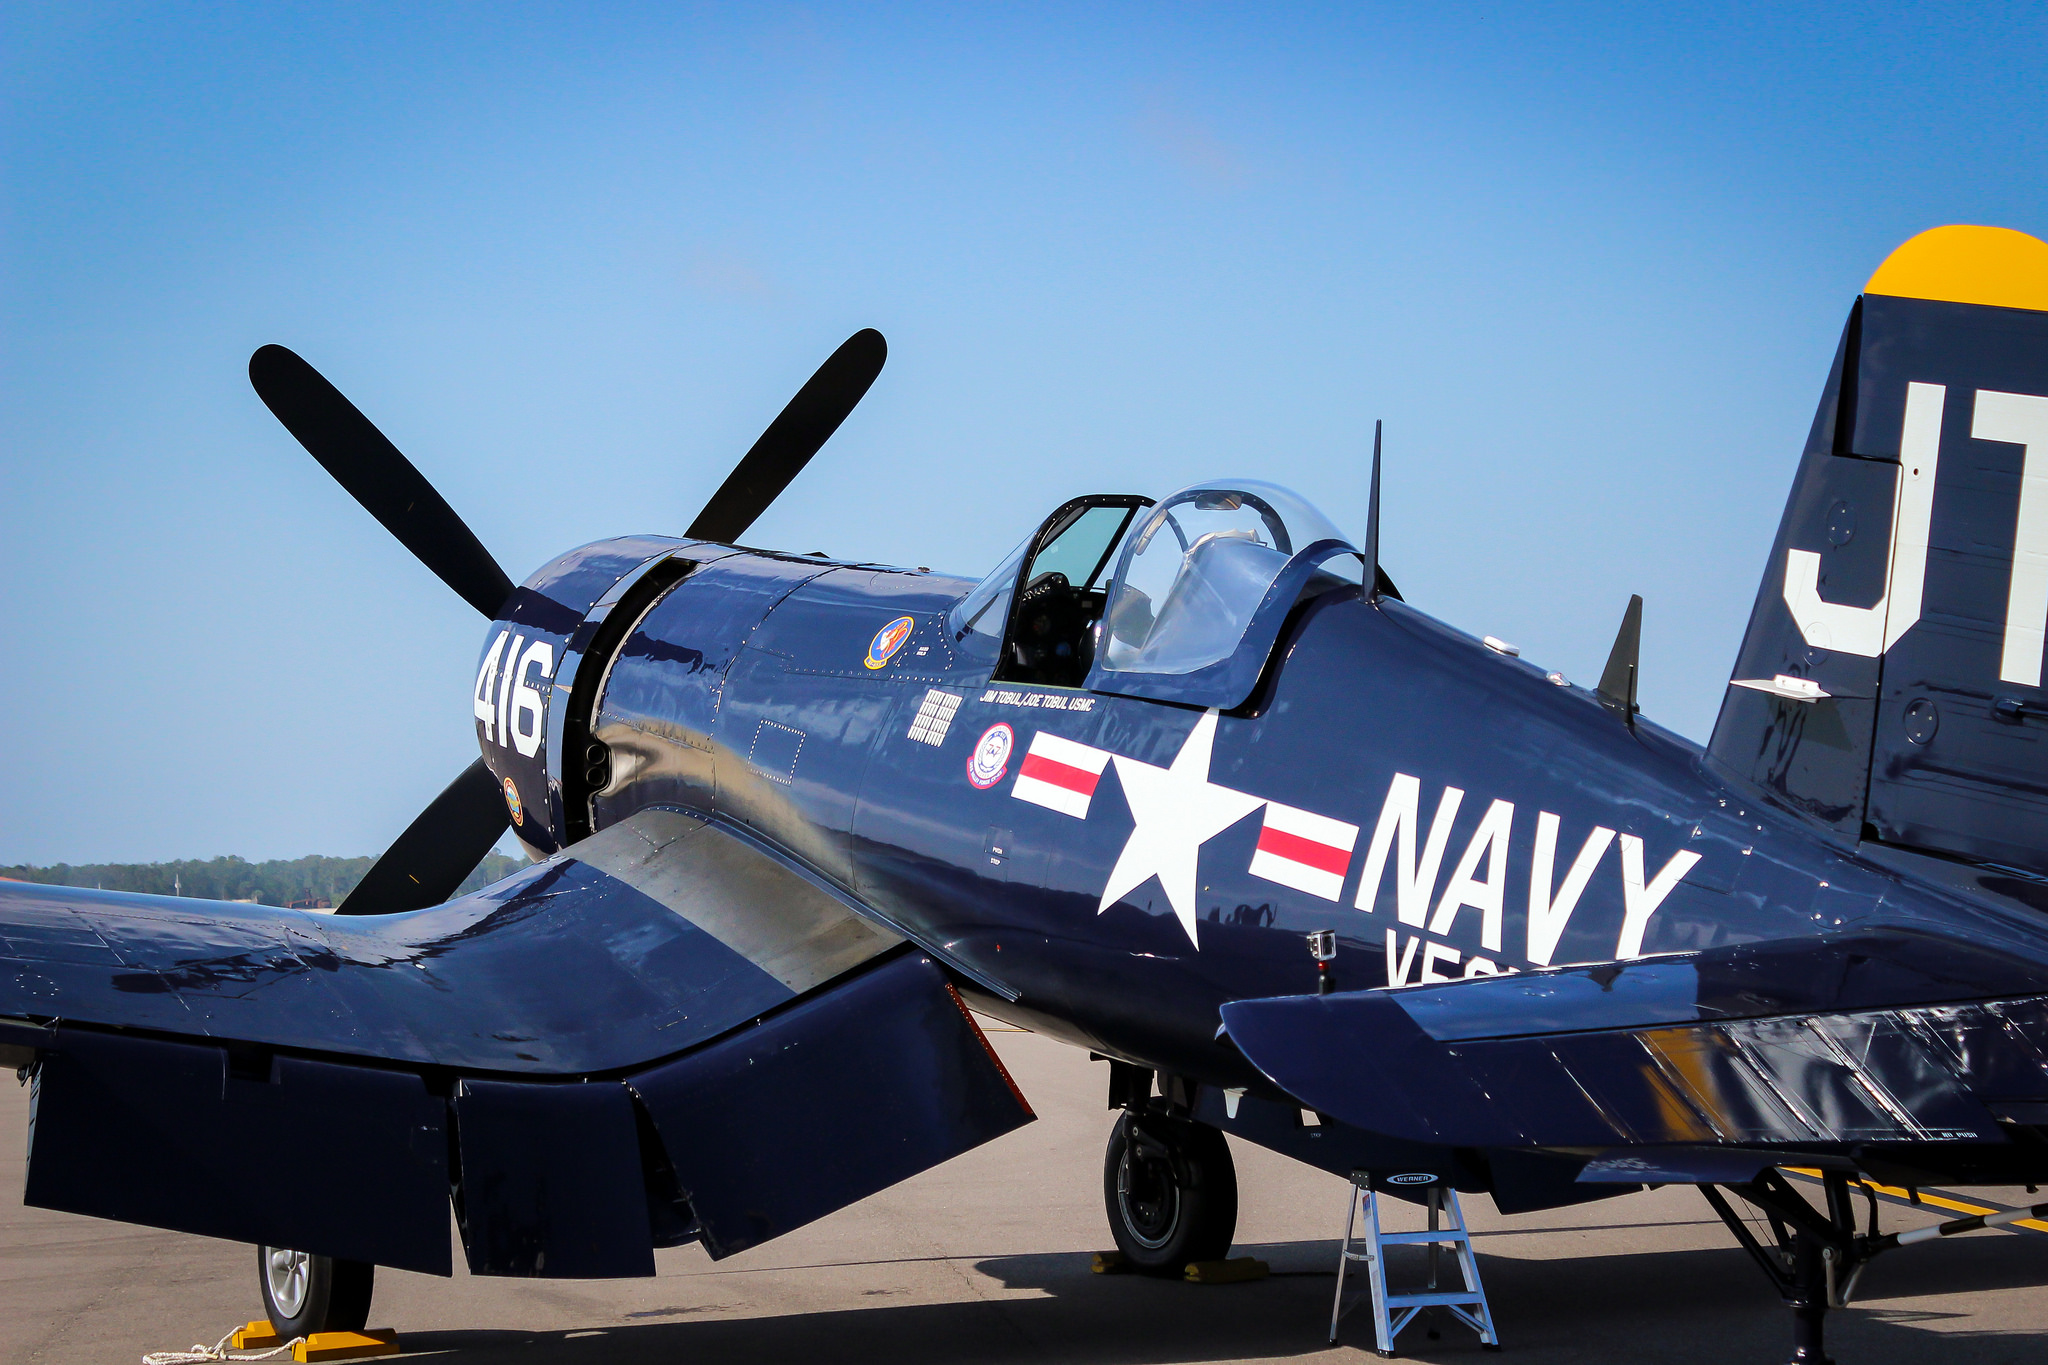
\includegraphics[width = 0.8\linewidth]{corsair_image_frontpage.jpg}

        \vspace{1cm}
    \end{center}

    \begin{flushleft}
        Année Académique 2023-2024

        NX22 - Alexandre Detienne - Décembre 2023
    \end{flushleft}
\end{titlepage}

\newpage
\tableofcontents

\newpage
\section{Introduction}
Le Chance Vought F4U Corsair, dit "Corsair", est un avion fabriqué par l'entreprise Vought pour la US Navy qui a marqué la seconde guerre mondiale. Conçu à la fin des années 1930 dans le but de servir principalement en tant qu'appui aérien lors des batailles navales, cet avion a été pensé pour pouvoir être transporté sur des porte-avions. Il est équipé d’un moteur à double étoile de 18 cylindres (2000 chevaux). Ce sont ces objectifs qui ont donné au Corsair sa forme très reconnaissable, à savoir des ailes pliables en forme de W (aussi appelée "ailes de mouette inversée").

\end{document}